\documentclass[12pt,a4paper,twoside]{article}

\usepackage[utf8]{inputenc} 
\usepackage{amsmath,amsfonts,amssymb} 
\usepackage{float} 
\usepackage{caption}
\usepackage{booktabs}
\usepackage{pgfplots}
\pgfplotsset{compat=1.18}
\usepackage{tikz}
\usetikzlibrary{calc,fit,angles,quotes,intersections}
\usepackage{adjustbox}
\usepackage[style=numeric,sorting=none]{biblatex}
\addbibresource{references.bib}
\usepackage{array}
\usepackage{multirow}
\usepackage{longtable}
\usepackage{tabularx}
\newcolumntype{Y}{>{\centering\arraybackslash}X}
\usepackage{siunitx}
\usepackage{microtype}
\usepackage{multicol}
\usepackage{listings}
\usepackage{xcolor}

% الروابط التفاعلية
\usepackage[hidelinks]{hyperref}

\usepackage[a4paper]{geometry}
\geometry{
  top=1in,
  bottom=1in,
  inner=1.25in,   % الهامش الداخلي (للتجليد)
  outer=1in        % الهامش الخارجي
}

% إضافة الصور
\usepackage{graphicx}


%لإضافة اسمك في نهاية الورقة 
\usepackage{fancyhdr}
\pagestyle{fancy}
\renewcommand{\headrulewidth}{0pt} % لإزالة الخط من الأعلى
\fancyhf{}% مسح الرأس والتذييل
%\fancyhead[L]{\textbf{Chapter 4 : Numerical solution of ordinary differential equations.}}
%\fancyfoot[R]{\textbf{Mezhoud maroua}} % اسمك في رأس الصفحة على اليسار
%\fancyfoot[C]{\thepage} % رقم الصفحة في الأسفل بالوسط

\usepackage{amsmath}
\usepackage{siunitx}
\usepackage{enumitem}


\begin{document}


\begin{titlepage}

\centering

\begin{flushleft}
    
\includegraphics[width=0.18\textwidth]{footer-logo.png}
\end{flushleft}

\vspace{1cm}

{\Large \textbf{Mohamed El Bachir El Ibrahimi University of Bordj Bou Arréridj} \par}

{\large Faculty of Science and Technology \par}

{\large Department of Materials Science \par}

{\large Undergraduate Programme (LMD) – Physics – Year 2\par}
   
{\large Course: Geometrical and Physical Optics\par}

{\large Topic: Wave Optics \par}
   
%تنسيق العنوان الرئيسي
%اجعليه في منتصف الصفحة تمامًا، بإضافة \vspace*{\fill} قبله و \vspace*{\fill} بعده بدلًا من \vspace{2cm}.
%هذا يجعل العنوان في المنتصف العمودي تمامًا، وهو المطلوب غالبًا.
\vspace*{\fill}
{\Huge \textbf{Practical Work  N\textsuperscript{o}:4} \\ Fresnel Mirrors
\par}
\vspace*{\fill}


  {\large \textbf{Submitted by:} \\
Mezhoud maroua\\  
\par}

 
\vspace{1 cm}
    
    {\large \textbf{Supervised by:} \\ Dr. S. Mameri\par}
    {\large Group:2 \par}
    
\vspace{2 cm}
    % بالنسبة للتاريخ هو تاريخ تسليم التقرير 
    {\large Date of submission: \today \par}
   

    {\large Academic Year: 2025–2026 \par}  
    


% \vfill تعني:
%املأ كل المساحة العمودية المتبقية هنا، وادفع ما يلي إلى أسفل الصفحة
\vfill
    
\end{titlepage}



%(لصفحة preliminary page) بدون رأس ولا تذييل
\pagestyle{plain}

% بدأ الترقيم بالأرقام العادية (لأنها عربية يا حبيبي ، تاع الخوارزمي)
\pagenumbering{arabic}  % الترقيم بالأرقام
\setcounter{page}{1}    % نبدأ من 1


\begin{abstract}
This practical work investigates the interference phenomenon produced by a Fresnel mirror using a He--Ne laser source. 
The experimental setup allows the creation of two virtual, coherent light sources by reflection on two slightly inclined plane mirrors. 
The resulting interference fringes are observed on a screen, and the interfringe distance is measured. 
By analyzing the geometrical parameters and the fringe spacing, the wavelength of the laser light is determined. 
The measured wavelength is found to be approximately $\lambda \approx 6.3 \times 10^{-7}\,\text{m}$, in good agreement with the theoretical wavelength of the He--Ne laser, confirming the validity of the Fresnel mirror method.
\end{abstract}



% الفهرس 
\tableofcontents

\newpage 



\section{Introduction}

Measuring the wavelength of light is fundamental in optics, as it underlies wave phenomena such as interference, diffraction, and coherence. Among various methods, the Fresnel mirror experiment provides a simple and elegant way to generate two virtual, coherent light sources from a single point source. The interference pattern produced by these sources allows precise determination of the wavelength. 

This practical work employs a He--Ne laser and a Fresnel mirror setup to observe interference fringes and measure the interfringe distance. By analyzing the geometrical configuration and fringe spacing, the wavelength of the laser light is determined, demonstrating both the wave nature of light and the effectiveness of the Fresnel mirror method.

\section{Objectives}
The main objectives of this experiment are as follows:
\begin{itemize}
    \item To generate two virtual, coherent light sources by reflection of a point light source on a Fresnel mirror.
    \item To observe the interference pattern produced by the two virtual light sources.
    \item To measure the fringe spacing $d$ between successive interference fringes.
    \item To determine the wavelength $\lambda$ of the He--Ne laser light from the measured fringe spacing $d$.
\end{itemize}



\section{Theoretical Background}
The Fresnel mirror consists of two plane mirrors forming a very small angle with each other. 
When a point light source $S$ is placed in front of the mirrors, its reflections produce two virtual images $S_1$ and $S_2$.
Since both virtual sources originate from the same primary source, they are coherent.

The interference pattern observed on the screen results from the superposition of the waves emitted by $S_1$ and $S_2$.
The distance $d$ between successive bright fringes (interfringe) is given by:
\[
d = \frac{\lambda (L_1 + L_2)}{a}
\]
where:
\begin{itemize}
    \item $\lambda$ is the wavelength of the laser light,
    \item $a$ is the distance between the two virtual sources,
    \item $L_1$ is the distance between the virtual sources and the projection lens,
    \item $L_2$ is the distance between the projection lens and the observation screen.
\end{itemize}

The separation $a$ between the virtual sources is determined from the geometrical projection:
\[
a = A \frac{L_1}{L_2}
\]
where $A$ is the distance between the images of the two virtual sources on the screen.



\section{Apparatus and Materials}
The experimental setup consists of the following elements:
\begin{itemize}
    \item A He--Ne laser source,
    \item A Fresnel mirror composed of two slightly inclined plane mirrors,
    \item Two converging lenses,
    \item An optical bench with a graduated scale,
    \item An observation screen,
    \item A ruler for measuring fringe spacing.
\end{itemize}



\section{Experimental Procedure}
The laser beam is first expanded using a converging lens so that its focal point acts as a quasi-point source.
This source is placed in front of the Fresnel mirror, generating two virtual coherent sources by reflection.

The interference fringes produced by the superposition of the two waves are observed on the screen.
The distance between successive bright fringes is measured.
A second lens projects the images of the virtual sources onto the screen, allowing the measurement of their separation.
All relevant distances along the optical bench are recorded.


\begin{figure}[H]
\centering
\fbox{%
  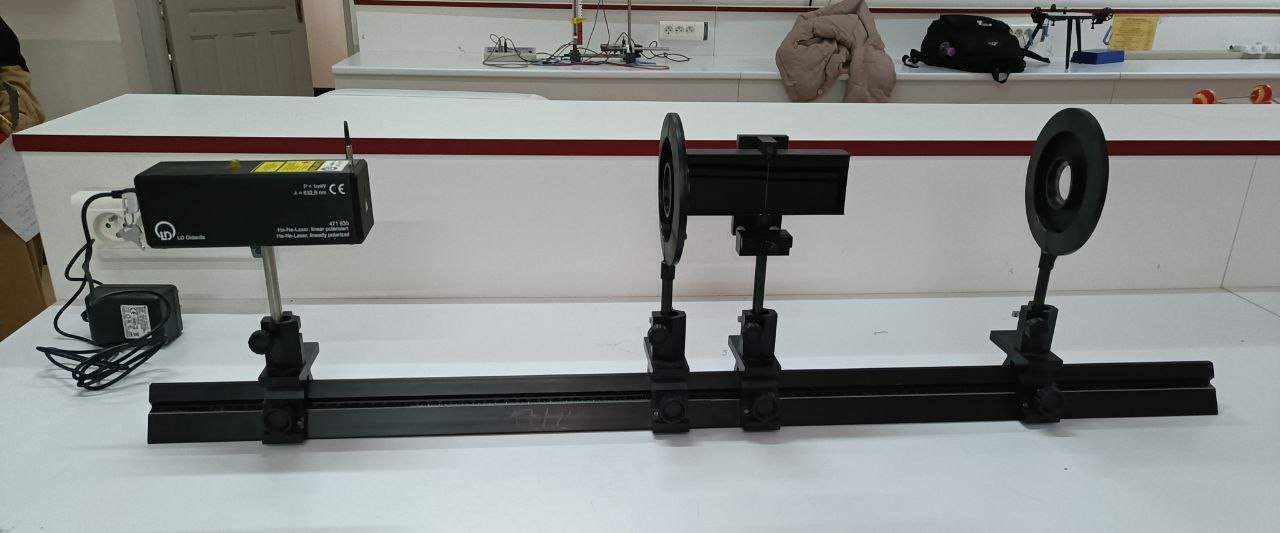
\includegraphics[width=\textwidth]{5915646851686271867.jpg}%
}
\caption{Experimental setup of the Fresnel mirror interference experiment.}
\label{fig:dioptre_plan_setup}
\end{figure}


\section{Results and Discussion}

\begin{table}[H]
\centering
\caption{Measured experimental values with uncertainties}
\begin{tabular}{l c c}
\toprule
\textbf{Quantity} & \textbf{Value} & \textbf{Uncertainty} \\
\midrule
Fringe spacing, $d$ & \SI{3.9}{mm} & \SI{0.1}{mm} \\
Image separation on screen, $A$ & \SI{4.3}{mm} & \SI{0.1}{mm} \\
Distance source to lens, $L_0$ & \SI{22.7}{cm} & \SI{0.1}{cm} \\
Distance lens to screen, $L_2$ & \SI{230.5}{cm} & \SI{0.1}{cm} \\
\bottomrule
\end{tabular}
\label{tab:measured_values}
\end{table}

The focal length of lens (1) is:
\[
f = \SI{5}{mm} \pm \SI{0.1}{mm}
\]

The distance between the virtual sources and lens (2) is:
\[
L_1 = L_0 - f = \SI{22.2}{cm} \pm \SI{0.1}{cm}
\]

The separation between the virtual sources is:
\[
a = A \frac{L_1}{L_2} \approx \SI{0.41}{mm} \pm \SI{0.01}{mm}
\]

% حساب الطول الموجي مع خطأ التجربة
The wavelength of the laser light is then calculated using:
\[
\lambda = a \frac{d}{L_1 + L_2} \approx \SI{6.3e-7}{m} \pm \SI{0.2e-7}{m}
\]

The theoretical wavelength of a He--Ne laser is:
\[
\lambda_\text{theo} \approx \SI{632.8}{nm} = \SI{6.328e-7}{m}
\]

\textbf{Relative Error:}
\[
\text{Relative Error} = \frac{|\lambda_\text{exp} - \lambda_\text{theo}|}{\lambda_\text{theo}} \times 100\% \approx 0.45\%
\]

\bigskip

\textbf{Discussion:}  

- The experimentally measured wavelength $\lambda_\text{exp}$ is very close to the theoretical value $\lambda_\text{theo}$, with a relative error of less than 0.5\%.  
- The uncertainty in the measurement is mainly due to the precision of the instruments:
    \begin{itemize}
        \item Ruler for measuring fringe spacing: $\pm 0.1$ mm
        \item Optical bench scale: $\pm 0.1$ cm
        \item Lens focal length: $\pm 0.1$ mm
    \end{itemize}
- Combining these uncertainties gives an estimated error in the wavelength of about $\pm 0.2 \times 10^{-7}$ m.
- Overall, the results confirm the validity of the Fresnel mirror method for measuring the wavelength of coherent light.

\section{Conclusion}
This practical work successfully demonstrated the interference phenomenon using a Fresnel mirror, highlighting the wave nature of light. 
By reflecting a single He--Ne laser source on two slightly inclined plane mirrors, two coherent virtual sources were generated, producing a clear interference pattern on the observation screen. 
Careful measurements of the interfringe distance, along with the precise determination of geometrical parameters of the setup, enabled an accurate calculation of the laser wavelength. 
The experimentally obtained wavelength closely matches the theoretical value, confirming both the reliability of the Fresnel mirror method and the validity of the underlying wave optics principles. 
This experiment not only reinforces the fundamental concepts of coherence and interference but also illustrates the importance of meticulous measurement and analysis in experimental physics. 
Overall, it provides a thorough and instructive example of applying theoretical knowledge to practical optical investigations.


\end{document}





